% !TEX root = ../main.tex
\section{Moss Kin}\label{src::naenk}
\begin{linenumbers}
\DndDropCapLine{W}{e thought they were mindless}
\textit{savages, but they know what they're doing.
They ain't hiding from us, they're preparing an attack.
They're studying our movement, figuring out our tactics.
They're hunting us.}

\hspace*{\fill} --- Grigor, Drejeck expedition leader.

The moss kin, or naenks, are moss creatures that hunt in the dark, warm, and wet jungles of Drejeck.
They hunt for sustenance and to gather fresh corpses.

\subsection*{Short and tangled}
The naenks are mostly known for their strange reproduction.
They spawn from the corpses of hunted humanoids exposed to the nanust spores of the great tree Tekatsae.
The spores grow into moss, merging with the corpse's muscle tissue and flesh.
After a period of about two months, the corpse rises again, this time in the shape of a naenk.

The moss kin are a thin race.
Their height varies considerably, but they usually are slightly smaller than their birth corpse.
Their bodies mock a humanoid shape, made up by a mix of bone, flesh, vine, and moss.
They protect their fragile interior with thick layers of flora.

Naenks typically have a healthy green coloration, but their skin can be of any mix of colors between moldy blue, dark orange, gray, and even white.
Their eyes are of a white or yellow color, where a thick fluid hides their pupils from the eyes of others.

Naenks naturally grow leaves and mossy tendrils at the top of their heads that resemble hair, which can be of a black, brown, or yellow color.
They typically arrange this mock-up of hair in a simple topknot.

% Due to the duality of their bodies, naenks follow a very particular diet.
% They needs to regularly consume meat in order to maintain the corpse inside them.
% They also feed off nutrients from the soil to feed the vines and plants that surround this corpse.

\subsection*{Tribal Communities}
% A naenk also assists their communication with rhythmic tapping on their body and using a complex system of gestures.
% Apart from these, they can also speak telepathically when close to tsaneks or sovereigns, aiding their communication.

Naenks are organized in tribal units called bands.
Each band is lead by the strongest naenk, the chief, who commands alongside a tsanek shaman.
Naenk chiefs bear special spores that can be used to infect beasts in a manner similar to the Tekatsae tree.
They spawn a bestial moss creature known as nuen with this spores, who acts as a pet or mount to the chief.
When a naenk travels alone, it is usual for them to also grow these spores as well.

Naenks build and craft very little.
Their gear is simply what they loot, and they build simple structures by imitation.

Due to their odd appearance and homicidal reproduction, naenks are seen as something to fear.
They however are very bold, yet fear the strangest things due to superstition.

Strangely, if they remain inside Drejeck, a naenk will not need to carry a qualar to remain sentient.
This ability only works inside of the jungle however, and they quickly lose their sentience if they leave their home without a qualar.

\subsection*{History and Legends}
To become part of a band, an infant naenk needs to go through a unique ritual.
A tsanek shaman removes their thyroid cartilage, who then punctures an odd pattern of holes into it.
After fitting small wooden tubes into these holes, the cartilage is put back into its original place.
After healing, the naenk's voice becomes accompanied by an eerie whistling noise, which is used for communication and intimidation.

Later, the naenk joins a group of other would-be-warriors.
They leave the safety of the tribe to travel to the northern lakes of Drejeck.
In there they must hunt a whowie, a huge frog-like beast that preys on the moss kin.

While they are fierce beasts, whowies are very afraid of the naenks' whistling, aiding the latter in combat.
If the group succeeds, the bravest of the group will cut the whowie's tongue.
Upon returning to the village, the group becomes a new band, and the owner of the tongue becomes the band's chief.

\subsection*{Call to Adventure}
A naenk rarely leaves the Drejeck jungle in which they are born.
However, many reasons can spark the need for a naenk or an entire band to abandon their home.
A band may leave engaging on a quest, as commanded by Tekatsae itself, or in shame after failing in one.
The most common bands abandoning the tribe are those that failed on their initiation rite, culled by the vicious whowie.

While in groups they may be savage, individual naenks are not completely insensitive people.
It is not too rare for a naenk to abandon their tribe in search for a different life.
Discontent with their chief, tiredness from their class system, or mere curiosity of the outside world count among the most common reasons for a naenk to travel by themselves.

% Only known among the naenk and the tsanek is the fact that a huge qualar lies inside the tree itself, which imbues the colossal plant with sentience.
% How this object ended up inside the tree is unknown, but it is thought among them that the tall one cter-rheth is looking to recover it.
% Due to the fact that the kin can't reproduce by themselves, they protect the tree with their lives and, under normal circumstances, won't allow anyone to even approach it.

There is an old legend of a courageous band that will one day sneak into Ctereth's lair and steal a huge bounty of qualars.
These will be used to grow a second tree, brother to Tekatsae, improving the kin's survival by a large margin.
Many groups have tried to become this band of legend, but none has returned thus far.

\begin{figure}[!b]
    \centering
    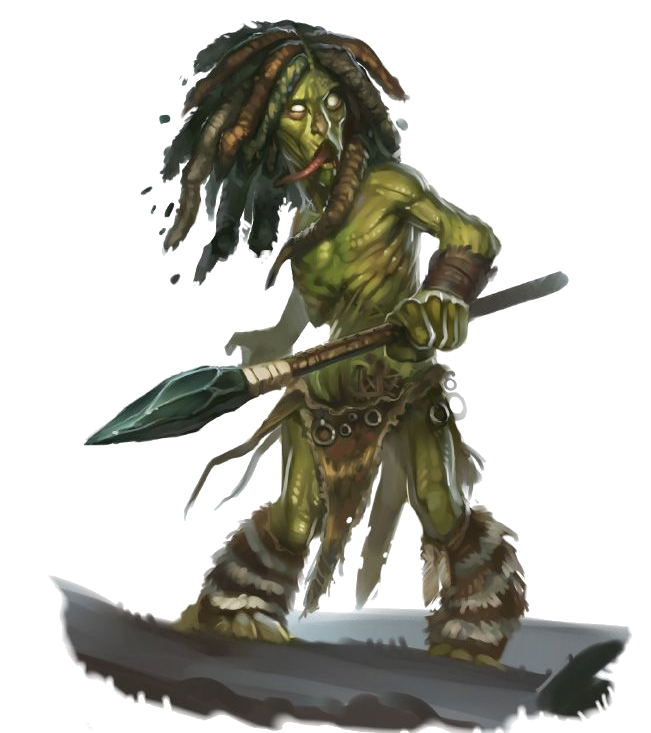
\includegraphics[width=0.48\textwidth]{03kins/img/15naenk_warrior.png}
\end{figure}

\subsection*{Naenk Names}
Naenks are born without names, and usually remain nameless most of their youth.
They reach social adulthood by earning a name, which is done either by becoming a warrior or accomplishing a major deed.

Many naenks live their whole lives unnamed.
While most accept this reality and become gatherers, it is not uncommon for the nameless to self-exile out of shame or discontent.

Knaenese is a very hard language to pronounce, so it's common for people of other kins to call naenks by a nickname or a simpler version of their name.

\paragraph{Names} Gantauda, Gesunt, Gunsedant, Hanhant, Hanseek needa, Hantadage, Huntge, Keena, Kegunseeda, Knaetseeknan, Knandage, Knudu, Kueqan, Nade, Naekuntge, Nega, Nelati, Seetun, Tsaegae, Tsege, Tsehant, Ukena.

\subsection*{Traits}
Your naenk character has an assortment of abilities, relating to their nature and surroundings.

\subparagraph{Ability Score Increase} Your Dexterity score increases by 2.

\subparagraph{Age} A naenk typically lives at most 30 years.
They are naturally mature right after being born and usually take less than a month to adapt to their society.

\subparagraph{Alignment} Naenks are organized creatures, used to following the rules of their communities.
Most tend towards the silver tide, especially those who haven't gained a name yet.

\subparagraph{Size} The moss kin come in very varied shapes and sizes.
They stand a tiny bit smaller than their birth corpse, but weight about half.
Your size and anatomy varies greatly depending on your birth corpse. \label{kin::naenk.size}

\subparagraph{Speed} Your base walking speed is 9 meters.

\subparagraph{Dual Nature} You are both humanoid and plant.

\subparagraph{Naenk claws} Because of your sharp claws, you have a base climbing speed of 9 meters.
In addition, your claws are natural weapons, which you can use to make unarmed strikes.
If you hit with them, you deal slashing damage equal to 1d4 + your Strength modifier, instead of the bludgeoning damage normal for an unarmed strike.

\subparagraph{Eat by Osmosis} While naenks prefer to eat meat by nature, you can mostly live off nutrients from the ground.
When in fertile land, you only need to eat once per week.
You can also eat more often if you choose to do so.

\subparagraph{Languages} You can speak, read, and write knaenese.
You can also speak, read, and write other language of your choice, but your pronunciation leaves much to be desired.

% Despite their lack of lips, the moss kin does speak a language, which is named Knaenese.
% Knaenese is a very simple, accommodating to their impaired speech.
% While a naenk can learn other languages, their pronunciation usually leaves much to be desired.

\subparagraph{Subraces} Naenks are most easily separated by their home - Gannag or Na'ane.

The most common of their kin, Gannagian naenks are the members of the tribes that surround the Tekatsae tree.
They have a very strong sense of community and an excellent capacity to work as a team.
Any one naenk will easily give their life without second thought for their people and for their way of life.

While all naenks are capable fighters, Gannagian naenk take on different jobs to fulfill different tasks.
The most common of these are the warriors, the hunters, and the gatherers.
Your subrace traits depend on which of these roles you take.

\subsubsection{Gannagian Warrior}
\subparagraph{Ability Score Increase} Your Strength score increases by one.

\subparagraph{Moldy Companion} As part of a long rest, you may contaminate a recently deceased beast with nanust spores.
To do this, you must succeed on a medicine ability check of DC 8 + the creature's number of hit dice.
If you succeed, the spores will settle into the beast, and the corpse rises as your nuen at the end of the long rest.

The nuen has the stats, abilities, and actions of the original beast, but its hit points and hit dice are cut in half.
It acts on its own volition and on its own initiative turn, but you can use an action to issue an order to it, which it follows to the best of its abilities.
It also gains the Plant Camouflage trait (page \pageref{trait::plantcamouflage}).

When travelling with one or more gannagian warriors, only the naenk with the highest Wisdom score can use this trait.

\subparagraph{Combat Training} The damage die of your claws is increased from a d4 to a d6.
Additionally, you can choose to add your Dexterity bonus rather than your Strength bonus to your attack and damage rolls.
% Trained and proficient in combat, you know the first rank of the \textbf{Armed Fighter} talent (page \pageref{tal::armedfighter}).

\subsubsection{Gannagian Hunter}
\subparagraph{Ability Score Increase} Your Constitution score increases by one.

\subparagraph{Plant Camouflage} You have advantage on Dexterity (Stealth) checks you make while in any terrain with ample obscuring plant life.

\subparagraph{Hunter's Guts} You are competent in the Survival skill.
Additionally, your base climbing speed is increased to 9.

\subsubsection{Gannagian Gatherer}
\subparagraph{Ability Score Increase} Your Intelligence score increases by one.

\subparagraph{Darkvision} Gatherers spend most of their life recollecting fungus underground, which provides you with an increased awareness in the dark.
You can see in dim light within 18 meters of you as if it were bright light, and in darkness as if it were dim light.
You can't discern color in darkness, only shades of gray.

\subparagraph{Seedspeech} Through sounds and touch, you can communicate simple ideas to living plants, and are able to interpret their responses as simple language.
Plants do not perceive the world in terms of sight, but most can feel differences in temperature, describe things that have touched them, as well as hear vibrations that happened around them (including speech).

\subsubsection{Na'anian Naenk}
Among the naenks that grow disillusioned with their tribes, many choose to pack their possessions and leave.
Among these self-exiled naenks, most usually choose to join the neighboring nation of Na'ane to live with their tsanek brothers.

These naenks drink a special beverage upon arrival known as nahan cooked by the nations sovereigns.
% NOTE: Nahan literally means "I-water" in Knaenese.
Nahan weakens the bond of the naenk with the Tekatsae tree, forcing them to attain a qualar to remain sentient.
% As a side effect, it also extends the naenk's life, pushing it to about 50 years.

\subparagraph{Ability Score Increase} You are learned the way of the tsaneks, and your Wisdom score increases by one.

\subparagraph{Rapport Spores} Your time among the tsaneks has allowed your body to adapt, and fungal growths are found all around your body.
You can extend rapport spores in a 4.5 meter radius as an action.
These spores go around corners and affect any creatures with an Intelligence score of 2 or more that aren't undead, constructs, or elementals.
Creatures affected by the spores realize the effect immediately, but those outside of range cannot notice it.
Affected creatures can communicate telepathically with one another while they remain within 9 meters of each other.
The effect lasts for 15 minutes.

\subparagraph{Noxious Spores} When a creature touches or hits you with a melee attack, you can choose to secrete noxious spores as a reaction.
The creature takes 1d6 poison damage if it isn't undead, construct, or elemental.
You can use this skill a number of times equal to your Constitution modifier (minimum of 2).
After expending all uses, you can't use this trait again until you complete a short rest.

\begin{figure}[!b]
    \centering
    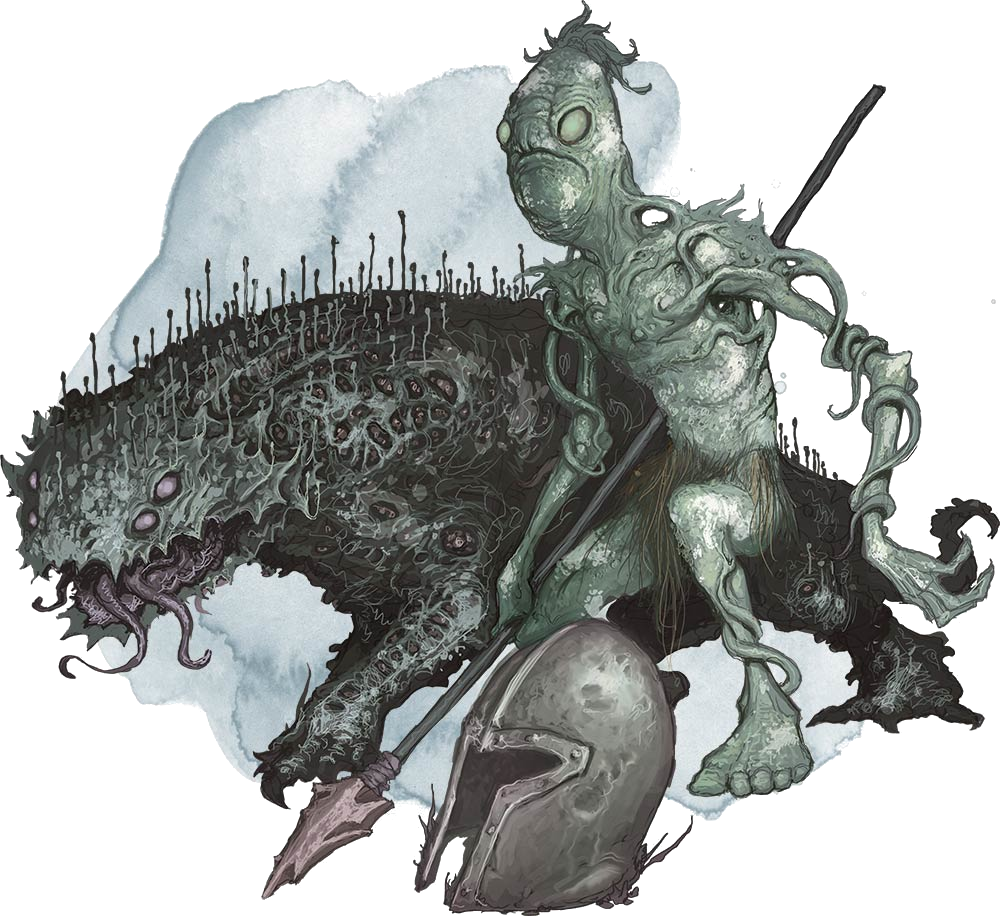
\includegraphics[width=0.48\textwidth]{03kins/img/15naenk_nuen.png}
\end{figure}

\end{linenumbers}

\newpage
